\section{Algorithms}
\subsection{Theory}
\subsubsection{Parallel PID controller}
% Translated from Garipov, Digital Control Systems 1, page 33.
The analog PID controller is an enchancement of the PI controller.
An aditional compoennt is assed to the PI sum.
It depends on the speed of change of the error but is expected to be zero at steady-state.
Here is how PID control looks like in the time domain:
\begin{equation}
    u(t) = K_p e(t) + K_p \frac{1}{T_i s} \int_0^{t_1} e(t) dt + K_p T_d \frac{d e(t)}{dt} = u_p(t) + u_i(t) + u_d(t)
\end{equation}
where $T_d$ is caleld derivative time constant.
\par
In state space the PID control law looks like this:
\begin{equation}
    u(s) = K_p e(s) + K_p \frac{1}{T_i s} + K_p T_d s e(s) = u_p(s) + u_i(s) + u_d(s)
\end{equation}
And for the transfer function (this is a \underline{parallel} structure PID) we have:
\begin{equation}
    W_{pid}(s) = \frac{u(s)}{e(s)} = K_p + K_p \frac{1}{T_i s} + K_p T_d s =
    K_p \Bigg[ \frac{T_i T_d s^2 + T_i s + 1}{T_i s}  \Bigg]
\end{equation}
The advantages of the PID controller include swift transient processes and reduced overshoot.
The main disadvantages is that when either the setpoint $u(t)$ or the Load Disturbance changes,
the effect is opposite - the derivative term strives for overshoot.
This is called 'set point kick' and is malitious \cite[p. 33] {garipov}.

\subsubsection{Anti-windup}
Among numerous practical applications, the permissible range of values for the controller output is limited.
For example, a mechanical valve cannot be opened wider than it's physical construction allows.
A triac-controlled heater cannot supply negative thermal energy.
When the control signal $u(t)$ exceeds the maximum possible control, the integral factor becomes ineffective.
\par
The most popular algorithms for aveliating this problem are \cite[p. 49] {garipov}:
\begin{itemize}
\item{Limmiting the magnitude of the integral sum in [$u^{max}, u^{min}]$}.
\item{Summing only on valid computed control (not clipped). }
\end{itemize}

\subsubsection{Plant models}
Some algorithms for tuning vontrollers rely on a model of the plant.
Others rely on observing a step response or stable oscilaltions state.
Thus, firstly the most commonly used models are examined \cite[p55]{garipov}.
\par
A two parameter model accounts for pure delay and first order plat dynamics.
It is used for integrating plants.
\begin{equation}
    W(p) = \frac{a}{L p} e^{- L p}
\end{equation}
,where:  \\
$L$ - pure time delay \\
$a$ - coefficient.
\par
A three parameter model is insted of aperiodic type.
\begin{equation}
    W(p) = \frac{K_0}{1 + T p} e^{-Lp}
\end{equation}
where:  \\
$L$ - pure time delay,  \\
$K_0$ - gain,  \\
$T$ - dominant time constant.

\subsubsection{PID tuning algorithms}
The \textbf{tangent method} is a graphical or computational algorithm.
A tangent line is constructed through the inflection point of the plant's step response.
By measuring the coordinats of the itnersection of this tangent with y or x axis,
the parameters of 2 or 3 parameter model are estimated \cite[p. 55]{garipov}.
\par
The \textbf{area-based method} for estimating coefficietnts of a 3 coefficient plat is a computational method.
Measured is the area between the setpoint and step response.
Also, measured is the area between the step response and x axis.
Solely by using those two measurements, the area-based method estimates 3 parameter models.
\par
\textbf{Optimization-based methods} can fit models of unspecified order.
\par
The \textbf{first method of Zigler-Nichols} is significant both for its simplicity and for its hystory value.
The algorithm defines mapping from coefficients in (5) to recommend p, i and d gains for the closed system.
Even among the plethora of modern methods, Zeighle-Nichols I remains a useful starting point for more complex methods, such as optimizing or self-tuning.
\par
The \textbf{second method of Ziegler-Nichols} is based on steering the plant into sustained oscillations.
The period and magnitude of the resultant oscillations are measured.
Together with the loop time and the amplitude of the relay, a second table provides suggestions on $K_p$, $T_i$. $T_d$.
This method is considered an improvement on the Ziegler-Nighols I method.
\par
\textbf{Astrom-Hagglund} also utilize the self-oscilating mode of target plant.
However, this method advies a different way of controlling the system into oscilations.
This relay-based method is believed to be more effective tahn ZN for stable or inert plants.
\par
Of course there exist numerous core complicated tuning algorithms, many of which propriatery.
Just to name a few: optimization of value function, neural networs, robust parameters for controlling stochastic plant.

\subsubsection{Digital PID controller}
One method relies on the following assumptions \cite[p. 88]{garipov}:
\begin{itemize}
\item[--]{$u_i(t)$ is estimated using second rectangle method}
\item[--]{$u_b(t)$ is estimated via first backwards finate difference.}
\end{itemize}
This is the non-recursive descrtiption of the controller:
\begin{equation}
    u(k) = K_p \Bigg[
    e(k) + \frac{T_0}{T_i} \sum_{i=1}^{k} e(i) + \frac{T_d}{T_0} (e(k)-e(k-1))
    \Bigg]
\end{equation}
\par
If the control law is to be computed by a digital device, a more efficient approach would be as follows.
Let us assume
$$ K_i \frac{K_p T_0}{T_i} $$
$$ K_d = \frac{K_p T_d}{T_0} $$
Then the PID controlelr can be written in the following rocursive format:
\begin{equation}
    u(k) = K_p e(k) + I(k) + K_d (e(k) - e(k-1))
\end{equation}
\begin{equation}
    I(k) = I(k-1) + K_i e(k),
    I(0) = 0
\end{equation}

% end of stupid theory
\subsection{PID implementation}
Used is a discret pid algorithm with parallel structure and integral windup.
The computer implementation expects proportional integral and derivative gains, as opposed to time constants.
Consequencly, the responsibility for translating from $T_i, T_d$ to $K_i, K_d$ falls to the client software, written by the author.

\subsection{Units of measure}
Because various physical and computational resources are performed in the system, unit conversions need to be carefully considered.
\par
We are constrained by the PID algorithm software to use 'int16\_t' values for input, output and coefficients.
Furthermore, coefficients are represented in 9s6 format i.e. $128 == 1.0$.
\par
Secondly, the temperature sensor interface library returns 'decicelsius\_t'.
This is an integral value of measured degrees celsius, multiplied by 10.
The accuracy of the thermometer is $0.5\si{\celsius}$
\par
Last constraint is the input to the triac control.
In an attempt to increase the resolution of the triac control algorithm as far as possible, the author has used the whole range of 'uint16\_t' values.
In other words, 0 corresponds to 0\% or 0\si{\volt} at the heater, and $2^16 \equiv 65536$ corresponds to 100\% or 230\si{\volt} at the heater.
\par
Apparently, the PID algorithm needs to read 'decicelsius\_t' and output 'uint16\_t', which is impossible.
One of the two units needs to be selected for the algorithm to work with, and the other - converted to/from.
The author has selected 'decicelsius\_t' as the more human-readable format.
Furthermore, no aditional precision is lost by using this shriked type.

\subsection{Nonlinearity}
The heating circuit is expected to exhibit good linearity.
However, the cooling process is both not under the control of the regulator, and extremely non-linear.
The author expects cooling to conform to the Stefan-Bolzman law of radiated thermal energy in free space:
$$ L = \frac{\sigma}{\pi}T^4 $$
If this is true, estimating a transfer function of the whole system is pointless.
The resulting linear system will be close to reality only for a very limited range of setpoints.

\subsection{Ziegler-Nichols sustained oscillations}
Initially, the Ziegler-Nichols algorithm for obtaining sustained oscillations and thus critical gain $K_u$ and critical period $T_u$ was attempted.
It was observed that if any oscillations are observed at all, their amplitude is lower than the absolute error in the system.
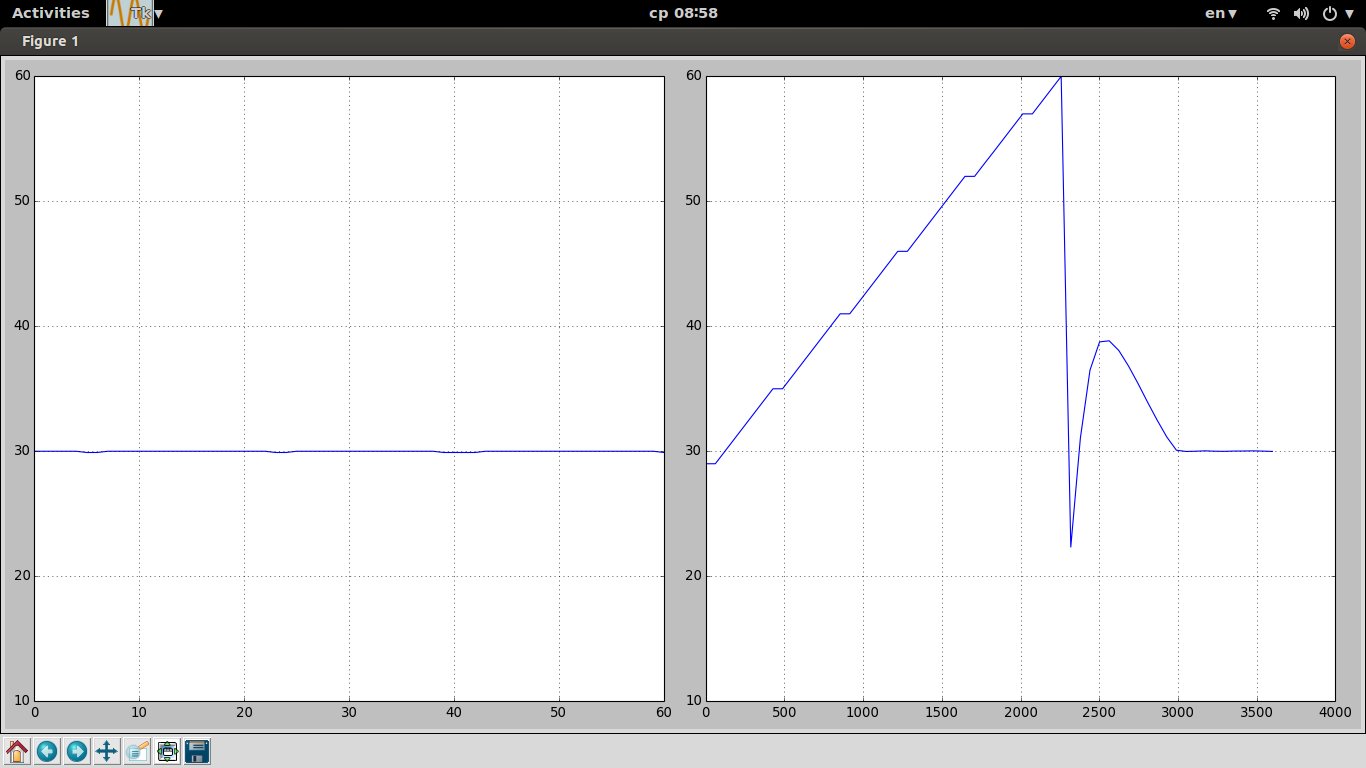
\includegraphics[width=0.85\textwidth]{../images/exp_gain100}~

\subsection{Astrom-Hagglund sustained oscillations}
Secondly, replacing the PID controller with a relay was attempted.
The relay acts as a sign function.
It was observed that again no sustained oscillations are exhibited by the system.
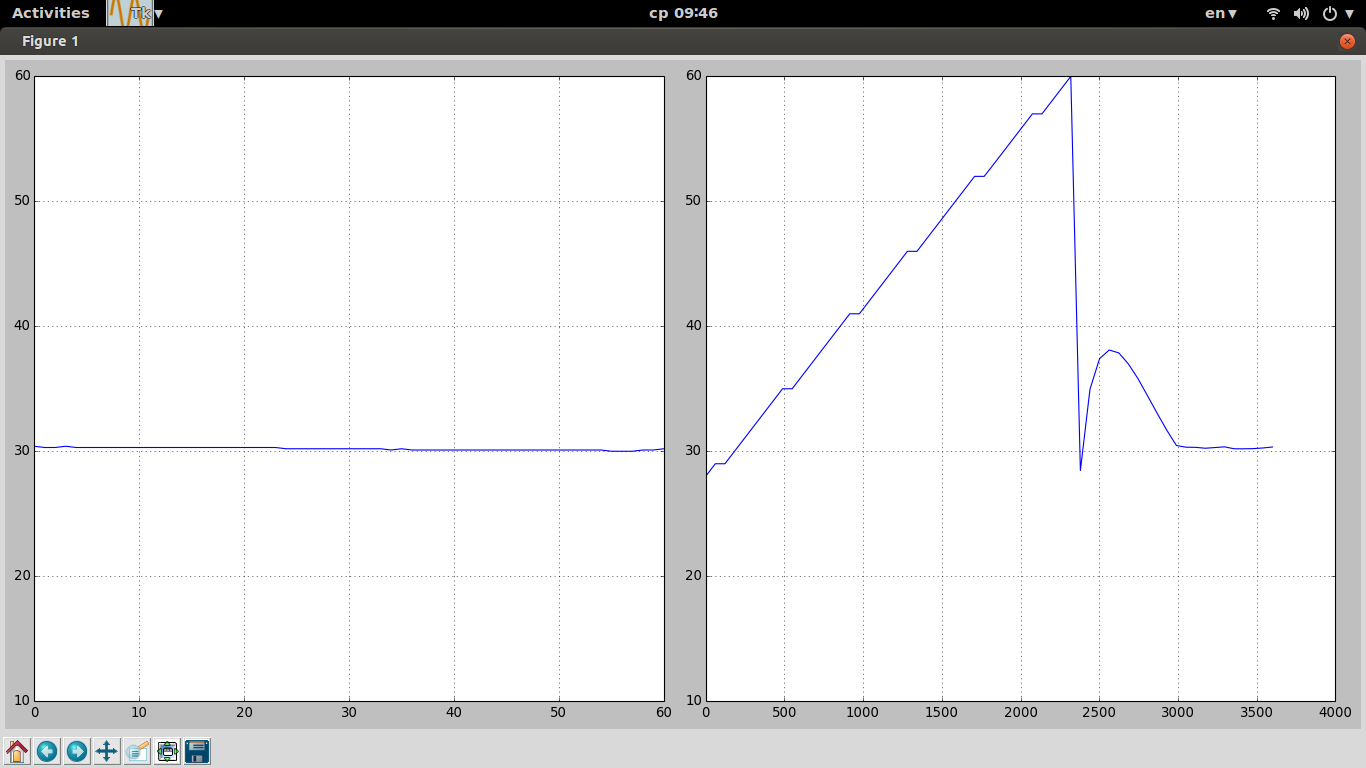
\includegraphics[width=0.85\textwidth]{../images/exp_relay}~

\subsection{Sampling rate correction}
Following advice in the literature, the author increased the control algorithm period to roughly $1/10$'th of the dominant open loop system time constant, namely to 60 seconds.
Finally sustained oscillations were observed.
\\
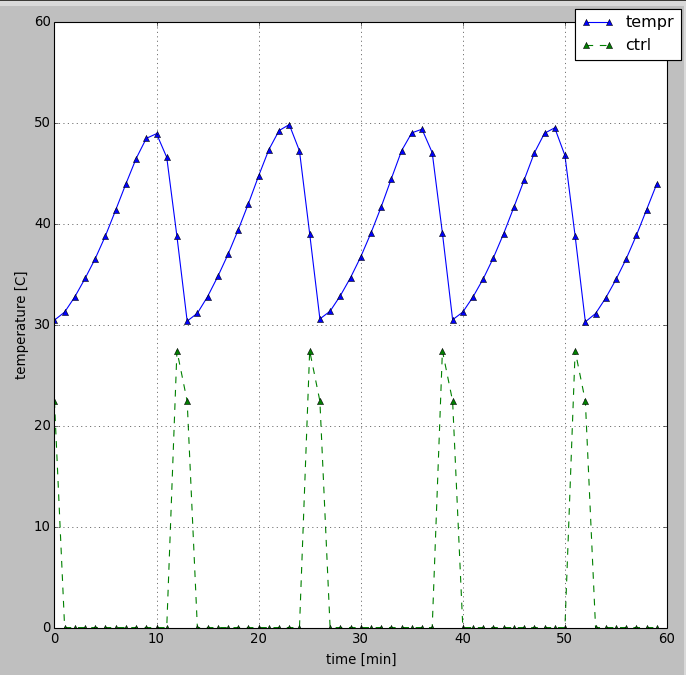
\includegraphics[width=0.85\textwidth]{../images/exp_relay_slow}~

\subsection{Peak detector}
A peak detector software module identifies local maxima and minima via 2 sample memory.
It is equivelend to 1-dimentional 2nd order casual digital filter.
During experiments it was established taht regardless of the inertial properties of the process, small local extrema (noise) twart the measurement.
\par
As the peak detector circuit is not expected to be low-latency, non-casual filter can be used for increased noise stability.
Proposed is a 6-sample memory filter of the type:

\par $
    y(k) = (x(k-3) \geq x(k)) \land (x(k-2) \geq x(k)) \land (x(k-1) \geq x(k)) \land
           (x(k+1) < x(k)) \land (x(k+2) < x(k)) \land (x(k+3) < x(k))
$ \par
where, \\
$y(k)$ - this function is 1 (true) during a local maximum, 0 (false) otherwise. \\
$x(k)$ - measured process output at k-th time period.
\\
This solution is superior to classical low-frequency because it does not introduce error in signal timestamps.
